\documentclass[border=4pt,12pt]{standalone}
% House style for redrawn exam diagrams (diagram-v4: 0.4pt lines, filled -latex arrows, fine dashes; stipple and hatching drawn as real dots/lines (no PDF/SVG patterns, so they render in every browser and at any scale); transparent background). Every figure \input's this.
\usepackage{amsmath,amssymb}
\usepackage{txfonts}
\usepackage{pdfrender,xcolor}
% \halo{text}: label on shading. The shading stops just around each letter's outline (a thin knock-out that follows the
% glyphs, like the papers' typesetting), never a box. Owner: "I don't want a box around the text".
\newcommand{\halo}[1]{\leavevmode\rlap{\pdfrender{TextRenderingMode=2,LineWidth=2.2pt,LineJoinStyle=1,StrokeColor=white,FillColor=white}#1}#1}
\usepackage{tikz,pgfplots}
\pgfplotsset{compat=1.18}
\usetikzlibrary{arrows.meta,calc,angles,quotes,patterns,patterns.meta,intersections,positioning,decorations.markings,shapes.geometric}
% Stipple and hatching are drawn as actual dots / lines clipped to the region (path picture), NOT as pattern fills:
% SVG <pattern> fills vanish or blur when browsers scale the image, so the owner could not see the shading.
% Each dot is a 0.72pt square (keeps SVGs small; reads as a dot at print size). Dots sit on one global staggered grid, so neighbouring regions line up.
\makeatletter
\newdimen\ex@x \newdimen\ex@y \newdimen\ex@xa \newdimen\ex@ya \newdimen\ex@xb \newdimen\ex@yb \newcount\ex@row
\def\exam@stipplecolor{black!75}\def\exam@dotr{0.42pt}\def\exam@dotgap{2.5}
\def\ex@rowdots{\ifdim\ex@x<\ex@xb \pgfpathrectangle{\pgfqpoint{\dimexpr\ex@x-0.36pt\relax}{\dimexpr\ex@y-0.36pt\relax}}{\pgfqpoint{0.72pt}{0.72pt}}\advance\ex@x by \exam@dotgap pt\relax\expandafter\ex@rowdots\fi}
\def\exam@stipple{%
  \pgftransformreset% dots are sized in real points even inside scaled pictures
  \pgfpointanchor{path picture bounding box}{south west}\ex@xa=\pgf@x \ex@ya=\pgf@y
  \pgfpointanchor{path picture bounding box}{north east}\ex@xb=\pgf@x \ex@yb=\pgf@y
  \pgfsetfillcolor{\exam@stipplecolor}\pgfmathsetmacro\ex@h{\exam@dotgap/2}%
  \pgfmathtruncatemacro\ex@r{floor(\ex@ya/\ex@h)-1}\ex@row=\ex@r\relax
  \ex@y=\ex@r\dimexpr\ex@h pt\relax
  \loop\ifdim\ex@y<\ex@yb
    \pgfmathtruncatemacro\ex@c{floor(\ex@xa/\exam@dotgap)-1}\ex@x=\ex@c\dimexpr\exam@dotgap pt\relax
    \ifodd\ex@row \advance\ex@x by \ex@h pt\fi
    \ex@rowdots
    \advance\ex@y by \ex@h pt \advance\ex@row by 1
    \ifnum\numexpr\ex@row-(\ex@row/4)*4\relax=0 \pgfusepath{fill}\fi% flush every 4 rows: bounded TeX memory, few clip copies in the SVG
  \repeat\pgfusepath{fill}}
\newdimen\ex@d
\def\exam@hatch#1{% #1 = 1 for /, -1 for \ ; lines 45 degrees, 3pt apart
  \pgftransformreset
  \pgfpointanchor{path picture bounding box}{south west}\ex@xa=\pgf@x \ex@ya=\pgf@y
  \pgfpointanchor{path picture bounding box}{north east}\ex@xb=\pgf@x \ex@yb=\pgf@y
  \ex@d=\dimexpr\ex@yb-\ex@ya\relax \ex@x=\dimexpr\ex@xa-\ex@d\relax
  \loop\ifdim\ex@x<\ex@xb
    \ifnum#1>0 \pgfpathmoveto{\pgfqpoint{\ex@x}{\ex@ya}}\pgfpathlineto{\pgfqpoint{\dimexpr\ex@x+\ex@d\relax}{\ex@yb}}%
    \else \pgfpathmoveto{\pgfqpoint{\ex@x}{\ex@yb}}\pgfpathlineto{\pgfqpoint{\dimexpr\ex@x+\ex@d\relax}{\ex@ya}}\fi
    \advance\ex@x by 4.24pt
  \repeat
  \pgfsetlinewidth{0.4pt}\pgfsetstrokecolor{black}\pgfusepath{stroke}}
\def\examstipple{\exam@stipple}\def\examhatch{\exam@hatch}\def\examsetstipplecolor#1{\def\exam@stipplecolor{#1}}\def\examsetdotgap#1{\def\exam@dotgap{#1}}
\makeatother
% (legacy pattern kept for old files)
% staggered stipple like the NESA papers' dotted shading
\pgfdeclarepatternformonly{exam stipple}{\pgfpointorigin}{\pgfqpoint{2.2pt}{2.2pt}}{\pgfqpoint{2.2pt}{2.2pt}}{%
  \pgfpathcircle{\pgfqpoint{0.55pt}{0.55pt}}{0.42pt}\pgfpathcircle{\pgfqpoint{1.65pt}{1.65pt}}{0.42pt}\pgfusepath{fill}}
\tikzset{
  every picture/.style={line width=0.6pt, >={Latex[length=2mm,width=1.3mm]}},
  curve/.style={line width=0.6pt},
  open arrow/.style={-{Latex[length=2mm,width=1.3mm]}},  % owner: filled -latex heads everywhere, no open chevrons
  aux/.style={dash pattern=on 2pt off 1.5pt, line width=0.6pt},
  shade/.code={\def\exA{#1}\def\exB{none}\ifx\exA\exB\else\pgfkeysalso{fill=black!18}\fi},
  shade/.default=on,
  shade dots/.style={fill=none, path picture={\examstipple}},
  stipple color/.code={\examsetstipplecolor{#1}},
  stipple gap/.code={\examsetdotgap{#1}},
  shade dense dots/.style={fill=none, stipple gap=1.6, path picture={\examstipple}},
  shade hatch/.style={fill=none, path picture={\examhatch{1}}},
  shade hatch reverse/.style={fill=none, path picture={\examhatch{-1}}},
  shade solid/.style={fill=black},
  pt/.style={circle, fill, inner sep=1.1pt},
  open pt/.style={circle, draw, fill=white, inner sep=1.1pt},
}
\pgfplotsset{
  exam axes/.style={axis lines=middle, axis line style={->}, xlabel={$x$}, ylabel={$y$},
    xlabel style={anchor=west}, ylabel style={anchor=south}, tick label style={font=\small},
    every axis plot/.append style={line width=0.6pt, black}, samples=200, clip=false,
    enlargelimits=false, axis on top},
}

\begin{document}
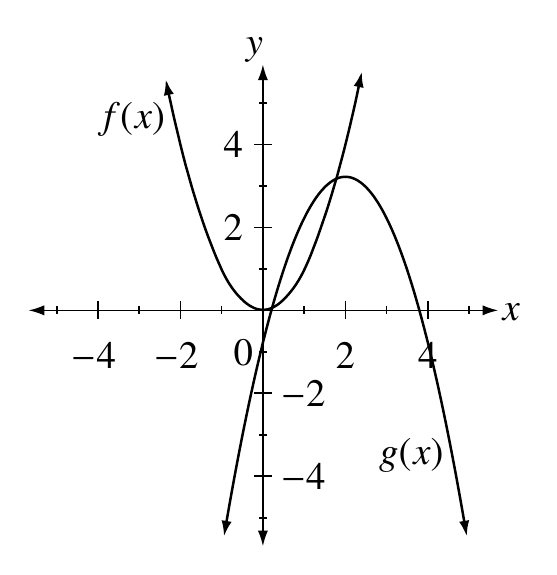
\begin{tikzpicture}[x=0.0127cm,y=-0.0127cm,font=\fontsize{14}{16.8}\selectfont]
\draw[<->] (12,286)--(482,286); \draw[<->] (246.5,522)--(246.5,40);
\draw (40.2,282.0)--(40.2,290.0);
\draw (242.5,493.5)--(250.5,493.5);
\draw (81.5,277.0)--(81.5,295.0);
\draw (237.5,452.0)--(255.5,452.0);
\draw (122.8,282.0)--(122.8,290.0);
\draw (242.5,410.5)--(250.5,410.5);
\draw (164.0,277.0)--(164.0,295.0);
\draw (237.5,369.0)--(255.5,369.0);
\draw (205.2,282.0)--(205.2,290.0);
\draw (242.5,327.5)--(250.5,327.5);
\draw (287.8,282.0)--(287.8,290.0);
\draw (242.5,244.5)--(250.5,244.5);
\draw (329.0,277.0)--(329.0,295.0);
\draw (237.5,203.0)--(255.5,203.0);
\draw (370.2,282.0)--(370.2,290.0);
\draw (242.5,161.5)--(250.5,161.5);
\draw (411.5,277.0)--(411.5,295.0);
\draw (237.5,120.0)--(255.5,120.0);
\draw (452.8,282.0)--(452.8,290.0);
\draw (242.5,78.5)--(250.5,78.5);
\draw[<->,line width=0.9pt] plot[smooth] coordinates {(149.2,54.9) (151.2,64.46) (153.3,74) (155.4,83.53) (157.5,93.05) (159.7,102.4) (162,111.9) (164.2,121.2) (166.6,130.7) (169,140) (171.6,149.2) (174.2,158.5) (176.9,167.7) (179.7,176.8) (182.6,186) (185.6,195) (188.7,204) (192,213) (195.4,221.8) (198.9,230.7) (202.6,239.3) (206.3,247.5) (210.3,255.1) (214.7,262.2) (219.5,268.6) (224.7,274.3) (230.2,279.2) (235.7,282.7) (241,284.8) (246.2,285.5) (251.2,285) (256.3,283.2) (261.8,279.9) (267.2,275.2) (272.5,269.5) (277.6,263) (282.2,256) (286.3,248.6) (290.1,240.6) (293.7,232.3) (297.1,223.5) (300.5,214.6) (303.7,205.5) (306.8,196.5) (309.9,187.4) (312.8,178.3) (315.6,169.1) (318.3,159.9) (321,150.7) (323.5,141.3) (326,132) (328.4,122.7) (330.7,113.4) (333,103.9) (335.2,94.51) (337.4,85) (339.5,75.61) (341.5,66.08) (343.5,56.54) (345.5,47)};
\draw[<->,line width=0.9pt] plot[domain=-0.945:4.945,samples=90,smooth] ({246.5+41.25*\x},{286-41.5*(3.22-(\x-2)*(\x-2))});
\node at (77.5,331) {$-4$};
\node at (160.0,331) {$-2$};
\node at (329.0,331) {$2$};
\node at (411.5,331) {$4$};
\node at (217,120.0) {$4$};
\node at (217,203.0) {$2$};
\node[anchor=west] at (255,369.0) {$-2$};
\node[anchor=west] at (255,452.0) {$-4$};
\node at (227,328) {$0$};
\node at (238,25) {$y$};
\node at (494,288) {$x$};
\node at (115,95) {$f(x)$};
\node at (395,431) {$g(x)$};\end{tikzpicture}
\end{document}
